% ISS presentation template
%
% Change history:
% 24.06.2010    J�rgen Ruoff        Initial creation
% 01.07.2010    Patrick H�cker      Generalization
% 02.07.2010    Patrick H�cker      Adjustment
% 15.11.2010    Patrick H�cker      Improvements
% 20.05.2011    Patrick H�cker      Add presentation type
% 06.01.2012	P. Hermannst�dter 	Adapted to ISS, small mods

% Insert your name here
\newcommand{\presenter}{Zhuowei Han}
\newcommand{\presentershort}{Z.Han}
\newcommand{\presenteremail}{} 		% can be accessed using \presenteremail

% Insert presentation title here
\newcommand{\presentationtitle}{Learning Deep Architectures for Pattern Recognition}
\newcommand{\shortpresentationtitle}{Deep Learning}

% Insert type of presentation here (or comment line), probably one of:
% Mitarbeitervortrag, Bachelor-Arbeit, Master-Arbeit, Bachelor thesis, Master thesis
\newcommand{\presentationtype}{---An introduction to Deep Neural Networks---}

% Insert presentation date here
\newcommand{\presentationdate}{05.06.2014}

% Uncomment the following line, if you write in English
%\newcommand{\lang}{german}

% Uncomment the following line, if you want to create handouts (setting to false does not work!)
% \newcommand{\handoutmode}{true}

% Load beamer class using LSS style
\input{presentation}

\usepackage{setspace}

% My commands:

% -----------------------------------------------------------------------------
% -----------------------------------------------------------------------------
\begin{document}
\lstset{basicstyle=\small\ttfamily,xleftmargin=15pt,language=Matlab,
        commentstyle=\color{green},showstringspaces=false,stringstyle=\color{magenta}\ttfamily}

% -----------------------------------------------------------------------------
% This is the title page
\begin{frame}[t,plain]
	\titlepage
\end{frame}


% -----------------------------------------------------------------------------
% Motivation slide
\begin{frame}[t]{Motivation}
\uncover<1->{
\textcolor{blue}{\Large Issues from Pattern Recognition}

\begin{minipage}[t]{0.48\linewidth}
\begin{figure}
\includegraphics{figures/patRec}
\end{figure}
\end{minipage}\hfill
\begin{minipage}[t]{0.48\linewidth}
	\begin{itemize}
		\itemsep40pt
		\item Optical Character Recognition 
		\item Object Recognition
		\item Speech Recognition / Speeker Identification / Emotion Recognition
	\end{itemize}
\end{minipage}
}

\end{frame}

\begin{frame}[t]{Motivation}
\uncover<1->{
\textcolor{blue}{\Large The usual approach}

\begin{minipage}[t]{0.48\linewidth}
\only<1-1>{
\begin{figure}
\includegraphics{figures/patternRecPipeline}
\end{figure}}
\only<2->{
\begin{figure}
\scalebox{0.7}{\includegraphics{figures/class2D}}
\end{figure}}
\end{minipage}\hfill
\begin{minipage}[t]{0.48\linewidth}
	\only<1-1>{
	\begin{figure}
		\scalebox{0.7}{\includegraphics{figures/class2D}}
	\end{figure}
	}	
	\only<2->{
	\begin{itemize}	
	\itemsep5pt	
		\item Feature engineering heavily dependent on application
						
		\begin{itemize}
			\item Natural clustering $P(X|Y = i)$ well separated
			\item Smoothness $x \approx y \rightarrow f(x) \approx f(y)$
		\end{itemize}
		
		\item Gap between feature engineering / classification
		\item Deep Architectures can bridge this gap by learning representations from high
			dimensional data
	\end{itemize}}
	
\end{minipage}
}

\end{frame}

% -----------------------------------------------------------------------------
% This is the table of contents. You can insert a motivation before or after this slide.
\begin{frame}
	\ifthenelse{\equal{\lang}{ngerman}}{
		\frametitle{Table of Contents}
	}{
		\frametitle{Table of Contents}
	}
	\tableofcontents
\end{frame}

% Add an extra slide at the beginning of each section while highlighting the current section
% Use \section* to skip the slide once or comment the following to skip all overview slides.
\AtBeginSection[]
{
	\begin{frame}<beamer>
		\ifthenelse{\equal{\lang}{ngerman}}{
			\frametitle{Table of Contents}
		}{
			\frametitle{Table of Contents}
		}
% 		\frametitle{\contentsname}
		\tableofcontents[currentsection]
	\end{frame}
}

%% =========
\section{Deep Architectures}
% -----------------------------------------------------------------------------
\begin{frame}[t]{Deep Architectures}

	\begin{itemize}
		\item Yoshua Bengio: A set of algorithms in machine 
			learning that use a set of non-linear transformations
			to model high-level abstractions and hidden dependencies in data
	\end{itemize}

\only<2->{
	\textcolor{blue}{\Large A natural Deep Architecture}	
	\begin{figure}
		\includegraphics{figures/brain}
	\end{figure}
	
	\begin{itemize}
		\item Can learn high-level abstractions from unlabeled data
		\item Representationally efficient 
	\end{itemize}}
	

\end{frame}

\begin{frame}[t]{Deep Architectures}
	\uncover<1->{
	\textcolor{blue}{\Large Deep Architectures in machine learning}	
	\begin{tabular}{c|c|c}
		Deep Belief Networks & Deep Neural Networks & Convolutional dNNs\\
		Geoffrey E. Hinton 2006 & Yoshua Bengio 2006 & others
	\end{tabular}\\}
	\vspace{0.5cm}
	\uncover<1->{
	\textcolor{blue}{\Large Evolution of Deep Neural Networks}	
	\begin{figure}
		\includegraphics{figures/timeLine}
	\end{figure}}
\end{frame}


%% =========
\section{Artificial Deep Neural Networks}
	\subsection{Concept}
	\begin{frame}[t]{Structure of Deep Neural Networks}
		\begin{figure}
			\psfrag{A}{$\underline{x}_k$}
			\psfrag{B}{$\hat{\underline{y}}_k$}
			\psfrag{I}{Input}
			\psfrag{O}{Output}
			\psfrag{C}{Layer $l$}
			\psfrag{D}{Layer $l+1$}
			\psfrag{E}{$\underline{z}^{(l)},\underline{a}^{(l)},\underline{b}^{(l-1)}, {\bf W}^{(l)}$}			
			\psfrag{F}{$\underline{z}^{(l+1)},\underline{a}^{(l+1)},\underline{b}^{(l)}, {\bf W}^{(l+1)}$}		
			\psfrag{P}{$\Phi$}			
			\psfrag{S}{$\Phi(x) = \frac{1}{1 + \mathrm{e}^{-x}}$}			
			\scalebox{0.6}{\includegraphics{figures/dNN}}
		\end{figure}
		
		\begin{minipage}[t]{0.48\linewidth}
		\begin{figure}
			Computing net-activation
			\begin{eqnarray}
				\underline{z}^{(l+1)}_k &=& {\bf W}^{(l)}\underline{a}^{(l)}_k + \underline{b}^{(l)} \nonumber \\
				\underline{a}^{(l+1)}_k &=& \underline{\Phi} \left ( \underline{z}^{(l+1)}_k \right ) \nonumber\\
				\hat{\underline{y}}_k &=& \underline{a}^{(ol)}_k \nonumber
			\end{eqnarray}
		\end{figure}
		\end{minipage}\hfill
		\begin{minipage}[t]{0.48\linewidth}
			\begin{itemize}
				\item Arbitrary non-linear mapping from $\underline{x}_k$ to  $\hat{\underline{y}}_k$ possible
				\item Relation $N \Leftrightarrow$ Complexity
				\item Deep Architectures $(l \uparrow)$ more efficient than shallow ones ($l\downarrow, N_l\uparrow$)
			\end{itemize}
		\end{minipage}
		
	\end{frame}
	
	\begin{frame}[t]{Determining the parameters}
		\textcolor{blue}{\Large Training objective}
			\begin{eqnarray}
				J({\bf W}, \underline{b}) &=& \sum_{\forall k} \frac{1}{2} ||\underline{y}_k - \hat{\underline{y}}_k||^2 + \frac{\lambda}{2} \sum_{\forall l} ||{\bf W}^{(l)}||_F^2 \\
				{\bf W}, \underline{b} &=& \arg \min_{{\bf W}, \underline{b}} J({\bf W}, \underline{b})
			\end{eqnarray}
			
		\textcolor{blue}{\Large Numerical minimization}		
		\begin{itemize}
			\item Gradient calculation with Backpropagation
			\item Stochastic gradient descent
			\item {\bf L}imited memory {\bf B}royden-{\bf F}letcher-{\bf G}oldfarb-{\bf S}hanno (L-BFGS)
		\end{itemize}	
	\end{frame}
	
	
	\subsection{Problems}
	\begin{frame}[t]{Problems}
		\begin{itemize}
			\item Optimization problem non-convex\\
			$\Rightarrow$ getting stuck in poor local minima
			\item Diffusion of gradients
		
		\begin{minipage}[t]{0.48\linewidth}
			\begin{figure}
				\psfrag{L}{Layer}
				\psfrag{G}{Gradient magnitude}
				\psfrag{S}{slow learning}
				\psfrag{F}{fast learning}				
				\scalebox{0.5}{\includegraphics{figures/gradDecay}}
			\end{figure}
		\end{minipage}\hfill
		\begin{minipage}[t]{0.48\linewidth}
			\begin{figure}
				\scalebox{0.6}{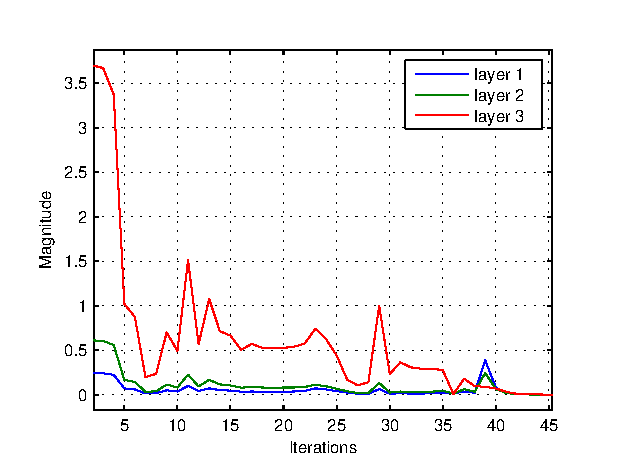
\includegraphics{figures/meanGradMag}}
			\end{figure}
		\end{minipage}
	\end{itemize}

	\end{frame}
	
\section{Unsupervised greedy layer-wise pre-training}
	
	
	\begin{frame}[t]{Unsupervised greedy layer-wise pre-training}
	
		\begin{itemize}
			\item Train the Deep Neural Network layer by layer (Hinton, Bengio)	
			\item Truncate network after first layer		
		\end{itemize}

		\begin{minipage}[t]{0.48\linewidth}
			\begin{figure}
				\psfrag{A}{$\underline{x}_k$}
				\psfrag{B}{$\underline{\hat{y}}_k$}
				\psfrag{I}{Input}
				\psfrag{C}{Coding}
				\psfrag{O}{Output}						
				\scalebox{0.7}{\includegraphics{figures/layerTraining01}}
			\end{figure}
		\end{minipage}
		
	\end{frame}
	
		\begin{frame}[t]{Unsupervised greedy layer-wise pre-training}
		
		\begin{minipage}[t]{0.48\linewidth}
			\begin{figure}
				\psfrag{A}{$\!\!\! \underline{a}_k^{(1)} = \underline{x}_k$}
				\psfrag{B}{$\underline{\hat{a}}_k^{(1)}$}
				\psfrag{I}{Input}
				\psfrag{C}{Coding}
				\psfrag{O}{Output}
				\psfrag{R}{Reconstruction}
				\psfrag{S}{Auto-Encoder}
				\psfrag{W}{${\bf W}^{(1)}$}
				\psfrag{V}{${\bf W}^{(1)T}$}
				\psfrag{E}{$\underline{b}_{enc}^{(1)}$}				
				\psfrag{F}{$\underline{b}_{rec}^{(1)}$}
				\scalebox{0.7}{\includegraphics{figures/layerTraining02}}
			\end{figure}
		\end{minipage}\hfill
		\begin{minipage}[t]{0.48\linewidth}
			\begin{itemize}					
				\item Reconstruction error
					\begin{equation}
						J_{AE} = \sum_{\forall k} \frac{1}{2} ||\underline{a}^{(1)}_k - \hat{\underline{a}}^{(1)}_k||^2 \nonumber
					\end{equation}				
				\item Small hidden layer: Learned subspace similar to PCA for linear activation $\underline{\Phi}(\cdot)$
			\end{itemize}
		\end{minipage}
		\vspace{1cm}
		\begin{itemize}
		\item Activation of the output layer
			$ \hat{\underline{a}}^{(1)}_k = \underline{\Phi} \left (  {\bf W}^T \underline{\Phi} \left ( {\bf W} \underline{x}_k  + \underline{b}_{enc} \right ) + \underline{b}_{rec} \right )$
		\end{itemize}
	\end{frame}
	
	\begin{frame}[t]{Unsupervised greedy layer-wise pre-training}
	\textcolor{blue}{\Large Force non-trivial solution}		
				\begin{itemize}
				\item Reduce number of hidden neurons
				\item Regularization
					\begin{equation}
						J_{reg} = ||{\bf W}||_F^2 
					\end{equation}
				\item Sparsity constraint
					\begin{eqnarray}
						\hat{\rho} &=& \frac{1}{m} \sum_{\forall k} [\underline{a}_k^{(2)}]_n \\
						J_{sp} &=& \sum_{\forall n} \mathrm{KL}(\rho||\hat{\rho}_n) \\
						\mathrm{KL}(\rho||\hat{\rho}_n) &=& \rho \log \frac{\rho}{\hat{\rho}_n}+ (1-\rho) \log \frac{1-\rho}{1-\hat{\rho}_n}
					\end{eqnarray}
				\item Overall cost
				\begin{equation}
					J = J_{AE}+ \lambda J_{reg} + \beta J_{sp}
				\end{equation}
					
				\end{itemize}
	\end{frame}
	
		
	\begin{frame}[t]{Unsupervised greedy layer-wise pre-training}
		\begin{itemize}
				\item Propagate input to second layer
				 \begin{equation}
					\underline{a}^{(2)}_k = \underline{\Phi} \left ( {\bf W}^{(1)} \underline{a}_k^{(1)}  + \underline{b}^{(1)} \right ) \nonumber
					\end{equation}
				\item Do pre-training of second layer
				\item ...
		\end{itemize}
		
			\begin{figure}
				\psfrag{A}{$\underline{a}_k^{(2)}$}
				\psfrag{B}{$\underline{\hat{a}}_k^{(2)}$}
				\psfrag{I}{Input}
				\psfrag{C}{Coding}
				\psfrag{O}{Output}
				\psfrag{R}{Reconstruction}
				\psfrag{S}{Stacked Auto-Encoder}
				\psfrag{W}{${\bf W}^{(2)}$}
				\psfrag{V}{${\bf W}^{(2)T}$}
				\psfrag{E}{$\underline{b}_{enc}^{(2)}$}				
				\psfrag{F}{$\underline{b}_{rec}^{(2)}$}
				\scalebox{0.7}{\includegraphics{figures/layerTraining03}}
			\end{figure}
		
				
	\end{frame}
	
			
	\begin{frame}[t]{Unsupervised greedy layer-wise pre-training}
		\begin{itemize}
				\item Add randomly initialized classification layer
				\item Perform dicriminative fine tuning, optimizing over weights and bias 
					terms of each stage
		\end{itemize}
		\begin{figure}
				\psfrag{A}{$\underline{x}_k$}
				\psfrag{B}{$\underline{\hat{y}}_k$}
				\psfrag{I}{Input}
				\psfrag{O}{Output}
				\psfrag{R}{Reconstruction}
				\psfrag{S}{Deep Neural Network}
				\scalebox{0.7}{\includegraphics{figures/layerTraining04}}
			\end{figure}
				
	\end{frame}

\section{Experiments}
	\subsection{Auto-Encoder for data compression}
	
	\begin{frame}[t]{Data compression}
	
	\begin{minipage}[t]{0.48\linewidth}
	\textcolor{blue}{\Large Experimental Setup}	
	\begin{itemize}
			\item Take 10 gray scale images
			\item Extract non-overlapping 8x8 patches
			\item Train Auto-Encoder for compression		
			\item Setup of the Auto-Encoder			
				\begin{itemize}
					\item 1 hidden layer $[64, 25, 64]$
					\item Training with 10.000 randomly selected patches
					\item LBFGS for optimization
					\end{itemize}
		\end{itemize}
	\end{minipage}\hfill
	\begin{minipage}[t]{0.48\linewidth}
		\begin{figure}
		\psfrag{A}{$\underline{x}_k$}
		\psfrag{B}{$\underline{\hat{x}}_k$}
		\psfrag{C}{Single stage Auto-Encoder}
		\psfrag{D}{Grayscale image}
			\scalebox{0.6}{\includegraphics{figures/compressionStructure}}
		\end{figure}
	\end{minipage}
	
	\end{frame}
	
	\begin{frame}[t]{Data compression}
	
	\begin{minipage}[t]{0.48\linewidth}
	\textcolor{blue}{\Large Original}	
		\begin{figure}
			\scalebox{0.4}{\includegraphics{figures/texture}}
		\end{figure}
	\end{minipage}\hfill
	\begin{minipage}[t]{0.48\linewidth}
	\textcolor{blue}{\Large Reconstructed}
		\begin{figure}
			\scalebox{0.4}{\includegraphics{figures/textureRec}}
		\end{figure}		
	\end{minipage}
	
	\end{frame}
	
	\begin{frame}[t]{Data compression}
	
	\begin{minipage}[t]{0.48\linewidth}
	\textcolor{blue}{\Large Learned features}	
			\begin{figure}
				\raggedleft
				\scalebox{0.5}{\includegraphics{figures/extractedFeatures}}
			\end{figure}

	\end{minipage}\hfill
	\begin{minipage}[t]{0.48\linewidth}
	\begin{itemize}
		\item Visualization
			\begin{itemize}
				\item Plot row vectors of ${\bf W}^{(1)}$, because:
			\end{itemize}
			\begin{equation}
				\underline{z}^{(2)}_k = {\bf W}^{(1)} \underline{x}_k + \underline{b}^{(1)} \nonumber
			\end{equation}

		\item The features are
		\begin{itemize}
			\item Corner features
			\item Edge features
			\item Texture features
		\end{itemize}
	\end{itemize}
	\end{minipage}
	
	\end{frame}
	
	\subsection{dNN for digit recognition}
	
	\begin{frame}[t]{Digit Recognition}
	
	\begin{minipage}[t]{0.48\linewidth}
	\textcolor{blue}{\Large Experimental Setup}	
	\begin{itemize}
			
			\item Using MNIST data base 
				\begin{itemize}
					\item 60.000 binar training images
					\item 10.000 binar test images
					\item 28x28 pixels
				\end{itemize}
							
			\item Setup of the dNN			
				\begin{itemize}
					\item 4 hidden layers $[784, 500, 200, 100, 10, 4]$
					\item Sigmoid activation function in all layers
					\item Tied-weights during layer-wise pre-training
					\item Cost / gradient calculation with all 60.000 training sets
					\item LBFGS for optimization 
				\end{itemize}
		\end{itemize}
	\end{minipage}\hfill
	\begin{minipage}[t]{0.48\linewidth}
		\only<1-1>{
		\textcolor{blue}{\Large First stage features}
		\begin{figure}
			\raggedleft
				\scalebox{0.5}{\includegraphics{figures/featuresMNIST}}
			\end{figure}}
	\end{minipage}
		
	\end{frame}
	
	
	\begin{frame}[t]{Digit Recognition}
			
		\begin{minipage}[t]{0.48\linewidth}
			\textcolor{blue}{\Large Last stage features}
			\begin{figure}
				\includegraphics{figures/digitPrototypes}
			\end{figure}
	%		\begin{equation}
%				\left [ \underline{x}^{(ol)} \right ]_n = \arg \max_{\underline{x}, s.t ||\underline{x}|| = 1} \left [ \underline{a}^{(ol)} \right ]_n \nonumber
%			\end{equation}
		\end{minipage}\hfill			
		\begin{minipage}[t]{0.48\linewidth}
		\textcolor{blue}{\Large Result}
			\begin{itemize}
				\item Clustering into 16 groups
				\item Learned representations are prototypes of handwritten digits			
				\item Recognition rate after discarding the last layer and performing
					discriminative fine tuning $98.2 \%$
			\end{itemize}
		\end{minipage}
	\end{frame}
	
	\subsection{Auto-Encoder for image reconstruction}

	\begin{frame}[t]{Auto-Encoder for image reconstruction}
	\textcolor{blue}{\Large Experimental Setup}	
	
	\begin{minipage}[t]{0.48\linewidth}
		\begin{figure}
		\psfrag{A}{$\underline{\tilde{x}}_k$}
		\psfrag{B}{$\underline{\hat{x}}_k$}
		\psfrag{C}{Single stage Auto-Encoder}
		\psfrag{D}{Distorted digits}
			\scalebox{0.6}{\includegraphics{figures/reconstructionStructure}}
		\end{figure}
	\end{minipage}\hfill
	\begin{minipage}[t]{0.48\linewidth}
		\begin{itemize}
		\uncover<1->{	
			\item Using MNIST data base 
			\item Adding random distortion which flips values at arbitrary positions
			$\underline{\tilde{x}}_k = \underline{x}_k + \underline{w}$
			}
			
			\uncover<1->{	
			\item Setup of the Auto-Encoder			
				\begin{itemize}
					\item 1 hidden layer $[784, 196, 784]$
					\item Sigmoid activation function in all layers
					\item Tied-weights
					\item Cost / gradient calculation with all 60.000 training sets
					\item LBFGS for optimization 
				\end{itemize}}
		\end{itemize}
	\end{minipage}
		
	\end{frame}
	
	\begin{frame}[t]{Auto-Encoder for image reconstruction}
	\textcolor{blue}{\Large Results}	
	
	\begin{minipage}[t]{0.48\linewidth}
		\begin{figure}
			\scalebox{0.6}{\includegraphics{figures/distorted01}}
		\end{figure}
	\end{minipage}\hfill
	\begin{minipage}[t]{0.48\linewidth}
		\begin{figure}
			\scalebox{0.6}{\includegraphics{figures/reconstruction01}}
		\end{figure}
	\end{minipage}
	
	Quadratic error:
	\begin{eqnarray}
		e_1 &=& \frac{1}{NL} \sum_{k = 1}^N || \underline{x}_k - \tilde{\underline{x}}_k ||^2 = 0.0873 \nonumber \\
		e_2 &=& \frac{1}{NL} \sum_{k = 1}^N || \underline{x}_k - \hat{\underline{y}}_k ||^2 = 0.0158 \nonumber 
	\end{eqnarray}	
		
	\end{frame}
	
	\begin{frame}[t]{Auto-Encoder for image reconstruction}
	\textcolor{blue}{\Large Results}	
	
	\begin{minipage}[t]{0.48\linewidth}
		\begin{figure}
			\scalebox{0.6}{\includegraphics{figures/distorted02}}
		\end{figure}
	\end{minipage}\hfill
	\begin{minipage}[t]{0.48\linewidth}
		\begin{figure}
			\scalebox{0.6}{\includegraphics{figures/reconstruction02}}
		\end{figure}		
	\end{minipage}
		
	Quadratic error:
	\begin{eqnarray}
		e_1 &=& \frac{1}{NL} \sum_{k = 1}^N ||\underline{x}_k - \tilde{\underline{x}}_k ||^2 = 0.2038 \nonumber \\
		e_2 &=& \frac{1}{NL} \sum_{k = 1}^N || \underline{x}_k - \hat{\underline{y}}_k ||^2 = 0.0239 \nonumber 
	\end{eqnarray}		
		
	\end{frame}
	
	\begin{frame}[t]{Auto-Encoder for image reconstruction}
		\textcolor{blue}{\Large Why this works (Vincent et al. 2010)}	
		\begin{figure}
			\includegraphics{figures/denoising}
		\end{figure}
		\begin{itemize}
			\item Auto-Encoder captures structure of input distribution
			\item Learns to map from low-probability regions to lower-dimensional
				high-probability regions
		\end{itemize}
	\end{frame}
	
\section{Summary}
	\begin{frame}[t]{Auto-Encoder for image reconstruction}
	\begin{itemize}
		\item Deep Architectures can bridge the gap between feature engineering and
			classification (representation learning)
		\item Deep Architectures can learn hierarchical abstractions from high-dimensional
			raw data and therefore enable non-local learning
		\item Greedy layer-wise pre-training results in an initialization of the network
			near a good local minima of the cost function
		\item Only unlabeled data is used during pre-training
		\item Stacked Auto-Encoders can be used for reconstruction of noisy data
			(Maybe even for reconstruction of MR-Images??)
	\end{itemize}	
	\end{frame}

\end{document}
